\chapter{Introduction}
\label{cha:intro}

It is astonishing how, based on the same genetic information coded into the DNA, cells in an organism can differentiate into a variety of specialized types with a multitude of different tasks.
Beginning with a single cell, a temporal, spatial and functional coordination determines the growth and body formation of eukaryotic organisms.
Depending on the cell state, only a fraction of genes is actively transcribed, while others remain repressed.
Acting as an additional regulatory layer, the epigenome describes a set of chemical modifications made to the DNA, controlling, inter alia, the activation and transcription of genes into RNA and ultimately proteins.
Present sequencing technologies and connected bioinformatics provide researchers with the tools to study sequence and epigenetic state down to single cell and single molecule resolution.
Starting 1990 and taking over a decade until completion, the human genome project incorporated an international team of researchers with the aim of deciphering for the first time the genetic blueprint to build a human being. 
Based on elementary sequencing technology, the outcome was already a nearly complete reference sequence including gene annotations.
Since then, the development of high-throughput, next-generation sequencing (NGS) technologies enabled studies of countless organisms, cell types and disease conditions. 
While being very reliable in terms of throughput and accuracy, sequenced fragments of at most few hundreds nucleotides in length still limit the readout from repetitive regions or resolution of long distance dependencies on a single molecule.




\section{Motivation}
\label{sec:intro:motivation}

Most recently, a third-generation of sequencing techniques is introducing new perspectives to the field of genome analysis by generating previously unattainable read lengths with averages in the tens of thousands of nucleotides. 
Still under active development and with frequent improvements, long-read sequencing provides new opportunities by, visually speaking, increasing the size of the puzzle pieces.
Moreover, direct sequencing of DNA and RNA molecules using the nanopore technology facilitates the detection of different types of base modifications.
Modern nanopore sequencing devices, producing large data sets within few days, open therefore a new field of research at the intersection of genomics, computer science and engineering. 
New data types, formats and error characteristics demand here the adaptation of existing and development of new algorithms for bioinformatic software.




\section{Genome Regulation}
\label{sec:intro:bio}

Most cell types of an eukaryotic organism contain a copy of the genetic code in form of folded DNA in the nucleus.
Virtually all mammals have diploid cells with homologous maternal and paternal copies, organized into chromosome pairs with the same genes at the same locations.
While the entire human genome comprises about three billion nucleotides in total, the longest continuous stretch of DNA is the first of 23 chromosome pairs with 247 million base pairs. 
To maintain its integrity and supporting the chromatin structure formation, the DNA is wrapped around octamers of histone proteins called nucleosomes (Fig. \ref{fig:intro:chromatin}).


\begin{figure}[h]
	\centering
	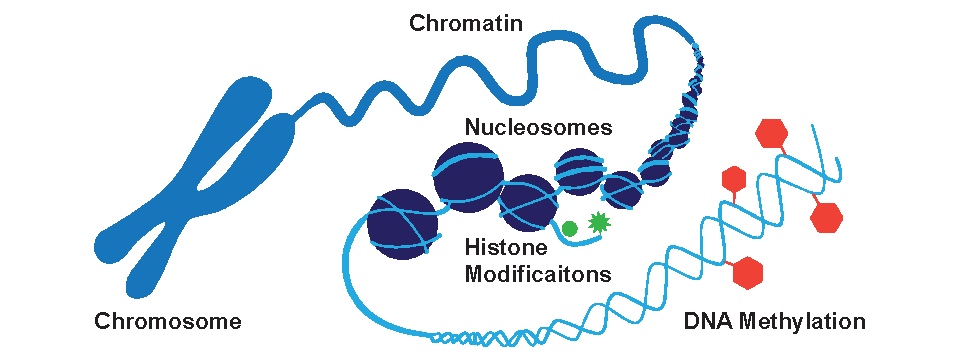
\includegraphics[width=1.0\textwidth]{figures/intro/chromatin.pdf}
	\captionsetup{format=plain}
	\caption[Chromosome to nucleotide structure]{The DNA of each chromosome is wrapped around histones, forming nucleosomes and the chromatin structure. Chemical modifications to histone tails and individual base pairs impact properties and cellular function (Adapted from \cite{zymo2020}).}
	\label{fig:intro:chromatin}
\end{figure}

The \textasciitilde 147bp of DNA directly twisted around each nucleosome is protected against physical access from for instance transcription factors (TFs). 
The dynamic positioning of nucleosomes is therefore part of the epigenetic regulation process during transcription and replication.
Accordingly, nucleosomes are enriched at compacted heterochromatin in mostly inactive genomic regions, while being depleted at regulatory elements such as enhancers, insulators and transcribed genes \cite{Klemm2019}. 
A growing number of chemical modifications to histone tails (H2A, H2B, H3 and H4) is reported to impact inter-nucleosomal interactions, but also leading to recruitment of proteins and complexes involved in transcription, replication and DNA repair \cite{Bannister2011}. 
A well characterized example is the methylation of lysine 79 on the H3 tail (H3K79me3) found at the transcription start sites (TSS) of active genes \cite{Lawrence2016}. 
To be further mentioned in this context are H3K4me3 marking active euchromatin, while H3K9me3 is indicating repressive heterochromatin.
Gene expression may be influenced by nearby active enhancer sites with enrichment of H3K27ac (acetylation).
Finally, repressed and bivalent promoters are modified with H3K27me3 and the combination of H3K4me4 and H3K27me3 respectively.

For embryonic development in mammals, the methylation of cytosine in the CpG-context (5-methylcytosine, 5mC) is a vital epigenetic modification. Prominent examples of its importance are the X-chromosome inactivation in females and genomic imprinting.
Furthermore, the DNA methylation is associated with the silencing of transposable elements, shows high levels over actively transcribed gene bodies and correlates with gene repression \cite{Greenberg2019}.
Throughout cellular reprogramming, \textit{de-novo} methylation of the DNA is primarily established by the DNMT3A and DNMT3B enzymes. 
During cell division, the methylation state on the nascent strand in the symmetric CpG-context is restored by the DNMT1 enzyme.
In absence of the maintenance methyltransferase, the 5mC modification is therefore passively lost during each round of replication, but can also be actively removed by oxidation through the TET methylcytosine dioxygenases.
There is a downside of cythosine methylation in the form of potential spontaneous deamination of 5mC, resulting in inherited C to T transitions and ultimately a depletion of CpG sites in mammalian genomes \cite{Holliday1993}. 
The human genome for example, contains only 29.4M CpGs instead of 188M as anticipated from the genome size. 
Thus, the conservation under evolutionary pressure underlines the importance of DNA methylation for mammals, while its function is still not yet fully understood.


On genome wide scale, methylation levels undergo two waves of reprogramming during embryonic development, of which the first one till stem cell state is illustrated in Fig. \ref{fig:intro:methylation}.


\begin{figure}[h]
	\centering
	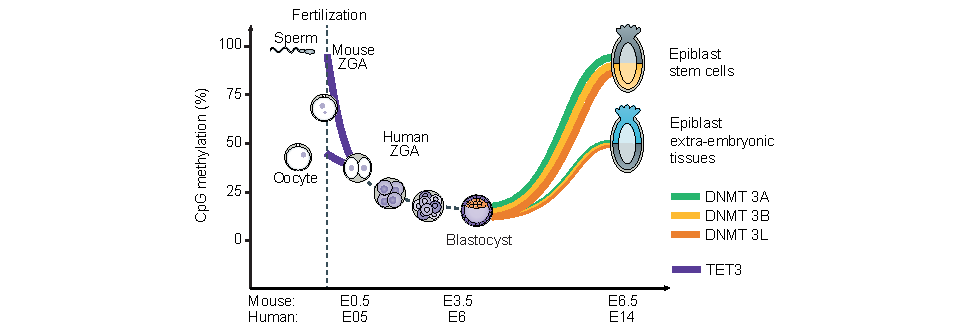
\includegraphics[width=1.0\textwidth]{figures/intro/methylation.pdf}
	\captionsetup{format=plain}
	\caption[DNA methylation reprogramming]{Reprogramming of CpG methylation during embryonic development: Following fertilization and zygotic genome activation (ZGA), mouse and human become actively demethylated by TET3. After blastocyst stage at mouse embryonic day E3.5, DNMT3A and DNMT3B establish \textit{de-novo} methylation under co-expression of DNMT3L. Extra embryonic tissues show a relative hypomethylation compared to the epiblast stem cells (Adapted from \cite{Greenberg2019}).}
	\label{fig:intro:methylation}
\end{figure}





repression of transposable elements LINE1 and IAP
hemi-methylation on genomic imprinting, ICRs
X-chromosome inactivation
high in actively transcribed gene bodies

de-regulation in cancer
tumor type identification based on methylation footprint

\begin{figure}[h]
	\centering
	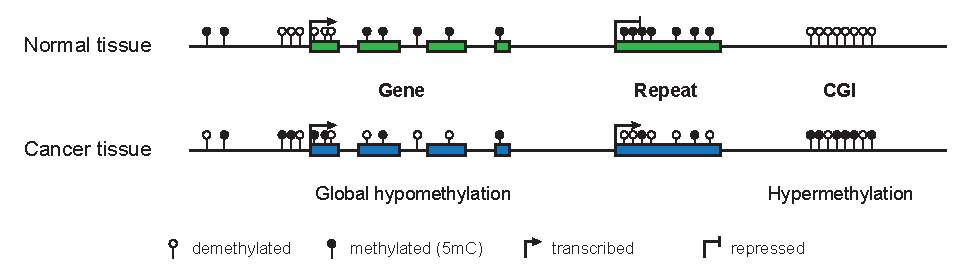
\includegraphics[width=1.0\textwidth]{figures/intro/cancer.pdf}
	\captionsetup{format=plain}
	\caption[DNA methylation in cancer]{}
	\label{fig:intro:cancer}
\end{figure}


The road ahead \cite{McGuire2020}




\section{Sequencing Technologies}
\label{sec:intro:sequencing}

\begin{figure}[h]
	\centering
	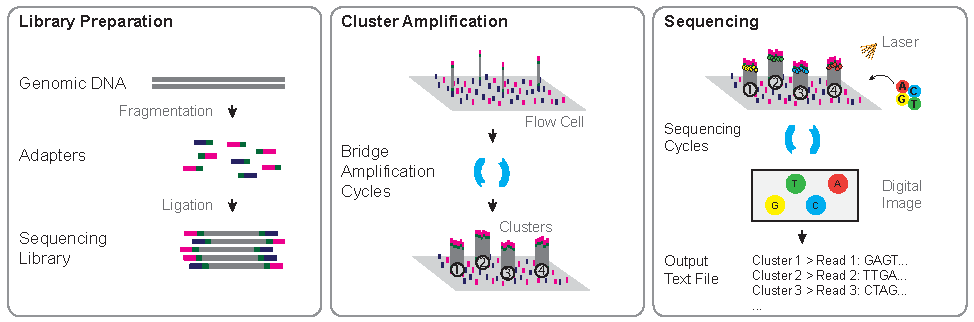
\includegraphics[width=1.0\textwidth]{figures/intro/sbs.pdf}
	\captionsetup{format=plain}
	\caption[Sequencing by synthesis]{Sequencing by synthesis}
	\label{fig:intro:sbs}
\end{figure}

Third revolution review \cite{Dijk2018}

\begin{figure}[h]
	\centering
	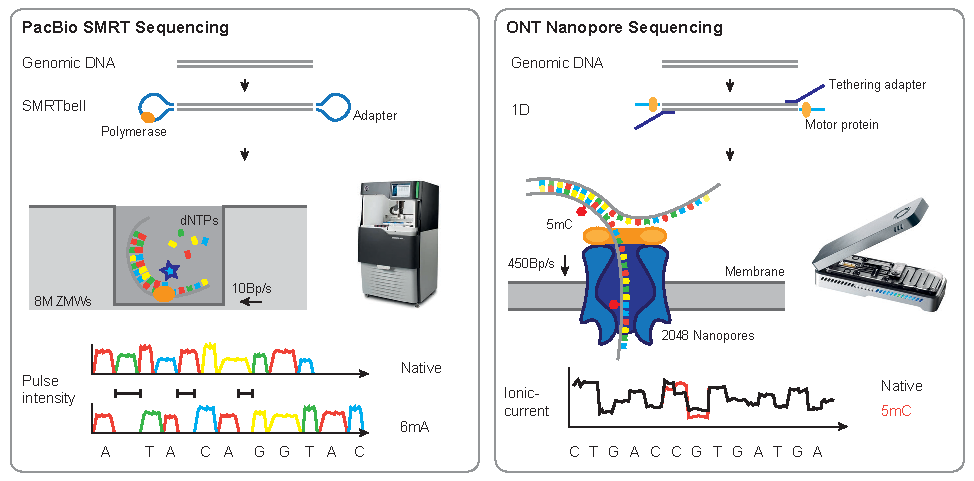
\includegraphics[width=1.0\textwidth]{figures/intro/long_read.pdf}
	\captionsetup{format=plain}
	\caption[Long read sequencing]{PacBio SMRT and ONT nanopore sequencing.}
	\label{fig:intro:longread}
\end{figure}

\begin{itemize}
    \item Sequencing
    \item Helene: "Easy to forget: but how to calculate a methylation rate from multiple reads and why minimum coverage. There is even a ref for 10X."
    \item Breifly generations, 1st, 2nd, 3rd ...
    \item Detail 3rd generation
    \begin{itemize}
        \item Briefly PacBio, Roche
        \item Detail ONT
    \end{itemize}
\end{itemize}

Among other devices distributed by Oxford Nanopore Technologies (ONT), the MinION in particular is gaining prominence. In brief, the nanopore sequencing process is based on guiding a nucleotide polymer through a pore inserted in a membrane while measuring a change in ionic current as a proxy signal over time. This signal is then interpreted to determine the underlying DNA or RNA sequence. The nanopore technology enables direct readout of sequences from individual DNA or RNA molecules, including base modifications, since no synthesis or amplification is required.




\section{Structure}
\label{sec:intro:structure}

Briefly describe the overall structure of the thesis, from literature to pipeline, signal processing and finally repeat detection.

%\textbf{Chapter \ref{sec:nanopype}} \\[0.2em]
%\blindtext

